
%-------------------------------------------------------------------------------
%							THIRD SECTION
%-------------------------------------------------------------------------------



\section{\textsc{Travaux et résultats}}


\subsection{Résultats en 1D}

\begin{frame}{Déplacement des noeuds d’un floe isolé (1)}

    \mycols{

        \mycol{50}{
            \myfigframe{Deplacement1D-Systeme.png}{Floe de glace 1D}

            \begin{figure}[!h]
                \begin{subfigure}[b]{0.45\textwidth}
                    \centering
                    \frame{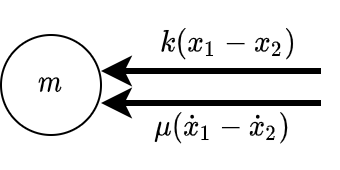
\includegraphics[width=\textwidth]{Deplacement1D-Masse1.png}}
                    % \caption{Sur la masse $m$ de gauche.}
                \end{subfigure}
                \begin{subfigure}[b]{0.45\textwidth}
                    \centering
                    \frame{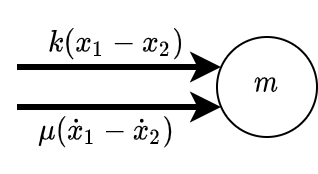
\includegraphics[width=\textwidth]{Deplacement1D-Masse2.png}}
                    % \caption{Sur la masse $m$ de droite.}
                \end{subfigure}
                   \caption{Bilan des forces}
            \end{figure}
        }

        \mycol{50}{
            Les équations de Newton-Euler:
            \begin{align*}
                \begin{dcases}
                m\ddot x_1 = - k(x_1 - x_2) - \mu(\dot x_1 - \dot x_2) \,,\\
                    m \ddot x_2 =  k(x_1 - x_2) + \mu(\dot x_1 - \dot x_2) \,. 
                \end{dcases}
            \end{align*}

            On préfère la forme générique:
            \begin{align*}
                \begin{dcases}
                    \dot{Y}(t)= E Y(t) \,,\\
                    Y_0 = Y(t_0) = (0,0,v_0,-v'_0)^T \,,
                \end{dcases}
            \end{align*}

            où :
            \begin{align*}
                E = \begin{pmatrix}
                    0 & 0 & 1 & 0 \\ 0 & 0& 0& 1 \\ -\frac{k}{m} & \frac{k}{m} & -\frac{\mu}{m} & \frac{\mu}{m} \\ \frac{k}{m} & -\frac{k}{m} & \frac{\mu}{m} & -\frac{\mu}{m}
                \end{pmatrix} \,,
                \text{ et } Y = \begin{pmatrix} x_1 \\ x_2 \\ \dot{x}_1 \\ \dot{x}_2 \end{pmatrix} 
            \end{align*}
        }
    }
    
\end{frame}


\begin{frame}[fragile]{Déplacement des noeuds d’un floe isolé (2)}

    \begin{columns}[onlytextwidth]

        \begin{column}{0.5\textwidth}
            \begin{lstlisting}[language=Python,caption=Code de simulation 1D]
    Y0 = np.array([0,0, v0, -v_0])
    t = np.linspace(0, tmax, N+1)
    
    def model(Y, t):
        return E @ Y

    Y = odeint(model, Y0, t)
            \end{lstlisting}
        \end{column}

        \mycol{50}{    
        \begin{theorem}[Convergence du modèle 1D isolé]
            Les déplacements $x_1$ et $x_2$ des noeuds du floe 1D convergent si et seulement si leurs vitesses initiales sont des vecteurs opposés.
        \end{theorem}
        }
    \end{columns}
    

    
    \begin{figure}[!h]
        \centering
        \begin{subfigure}[t]{0.45\textwidth}
            \centering
            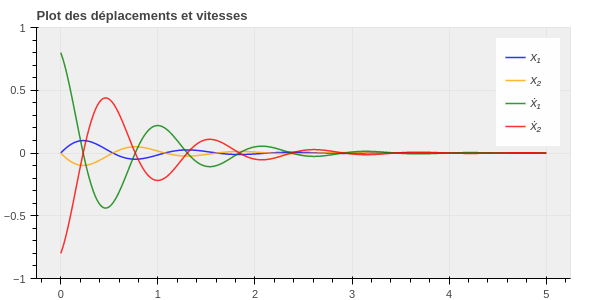
\includegraphics[width=\textwidth]{SimuDeplacement1D1.png}
            \caption{$v_0=v'_0 = 0.8$}
        \end{subfigure}
        \begin{subfigure}[t]{0.45\textwidth}
            \centering
            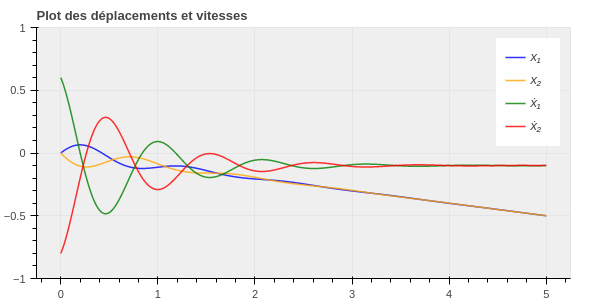
\includegraphics[width=\textwidth]{SimuDeplacement1D2.png}
            \caption{$v_0= 0.6$ et $v'_0 = 0.8$}
        \end{subfigure}    
        \caption{Simulation du déplacement d'un floe en 1D}
    \end{figure}

\end{frame}



